\ifx\wholebook\relax \else
% ------------------------

\documentclass{article}
%------------------- Other types of document example ------------------------
%
%\documentclass[twocolumn]{IEEEtran-new}
%\documentclass[12pt,twoside,draft]{IEEEtran}
%\documentstyle[9pt,twocolumn,technote,twoside]{IEEEtran}
%
%-----------------------------------------------------------------------------
%\input{../../../common.tex}
%
% loading packages
%

\RequirePackage{ifpdf}
\RequirePackage{ifxetex}

%
%
\ifpdf
  \RequirePackage[pdftex,%
       bookmarksnumbered,%
              colorlinks,%
          linkcolor=blue,%
              hyperindex,%
        plainpages=false,%
       pdfstartview=FitH]{hyperref}
\else\ifxetex
  \RequirePackage[bookmarksnumbered,%
               colorlinks,%
           linkcolor=blue,%
               hyperindex,%
         plainpages=false,%
        pdfstartview=FitH]{hyperref}
\else
  \RequirePackage[dvipdfm,%
        bookmarksnumbered,%
               colorlinks,%
           linkcolor=blue,%
               hyperindex,%
         plainpages=false,%
        pdfstartview=FitH]{hyperref}
\fi\fi
%\usepackage{hyperref}

% other packages
%--------------------------------------------------------------------------
\usepackage{graphicx, color}
\usepackage{subfig}
\usepackage{tikz}
\usetikzlibrary{matrix,positioning}

\usepackage{amsmath, amsthm, amssymb} % for math
\usepackage{exercise} % for exercise
\usepackage{import} % for nested input

%
% for programming
%
\usepackage{verbatim}
\usepackage{listings}
\usepackage{lipsum}
%\usepackage{algorithmic} %old version; we can use algorithmicx instead
\usepackage{algorithm}
\usepackage[noend]{algpseudocode} %for pseudo code, include algorithmicsx automatically
\usepackage{appendix}
\usepackage{makeidx} % for index support
\usepackage{titlesec}

\usepackage{fontspec}
\usepackage{xunicode}
\usepackage{fontenc}
\usepackage{textcomp}
\usepackage{url}
\usepackage{courier}

\titleformat{\paragraph}
{\normalfont\normalsize\bfseries}{\theparagraph}{1em}{}
\titlespacing*{\paragraph}
{0pt}{3.25ex plus 1ex minus .2ex}{1.5ex plus .2ex}

\lstdefinelanguage{Smalltalk}{
  morekeywords={self,super,true,false,nil,thisContext}, % This is overkill
  morestring=[d]',
  morecomment=[s]{"}{"},
  alsoletter={\#:},
  escapechar={!},
  literate=
    {BANG}{!}1
    {UNDERSCORE}{\_}1
    {\\st}{Smalltalk}9 % convenience -- in case \st occurs in code
    % {'}{{\textquotesingle}}1 % replaced by upquote=true in \lstset
    {_}{{$\leftarrow$}}1
    {>>>}{{\sep}}1
    {^}{{$\uparrow$}}1
    {~}{{$\sim$}}1
    {-}{{\sf -\hspace{-0.13em}-}}1  % the goal is to make - the same width as +
    %{+}{\raisebox{0.08ex}{+}}1		% and to raise + off the baseline to match -
    {-->}{{\quad$\longrightarrow$\quad}}3
	, % Don't forget the comma at the end!
  tabsize=2
}[keywords,comments,strings]

%% \lstdefinestyle{Haskell}{
%%   flexiblecolumns=false,
%%   basewidth={0.5em,0.45em},
%%   morecomment=[l]--,
%%   literate={+}{{$+$}}1 {/}{{$/$}}1 {*}{{$*$}}1 {=}{{$=$}}1
%%            {>}{{$>$}}1 {<}{{$<$}}1 {\\}{{$\lambda$}}1
%%            {\\\\}{{\char`\\\char`\\}}1
%%            {->}{{$\rightarrow$}}2 {>=}{{$\geq$}}2 {<-}{{$\leftarrow$}}2
%%            {<=}{{$\leq$}}2 {=>}{{$\Rightarrow$}}2
%%            {\ .}{{$\circ$}}2 {\ .\ }{{$\circ$}}2
%%            {>>}{{>>}}2 {>>=}{{>>=}}2
%%            {|}{{$\mid$}}1
%% }

% For better Haskell code outlook
\lstdefinelanguage{Haskell}{
  flexiblecolumns=false,
  basewidth={0.5em,0.45em},
  morecomment=[l]--,
  morekeywords={case, class, do, else, True, False, if, import,
    instance, module, type, data, deriving, where},
  literate={+}{{$+$}}1 {/}{{$/$}}1 {*}{{$*$}}1 {=}{{$=$}}1
           {>}{{$>$}}1 {<}{{$<$}}1 {\\}{{$\lambda$}}1
           {\\\\}{{\char`\\\char`\\}}1
           {->}{{$\rightarrow$}}2 {>=}{{$\geq$}}2 {<-}{{$\leftarrow$}}2
           {<=}{{$\leq$}}2 {=>}{{$\Rightarrow$}}2
           {\ .}{{$\circ$}}2 {\ .\ }{{$\circ$}}2
           {>>}{{>>}}2 {>>=}{{>>=}}2
           {|}{{$\mid$}}1
}[keywords,comments,strings]

% "define" Scala
\lstdefinelanguage{Scala}{
  morekeywords={abstract,case,catch,class,def,%
    do,else,extends,false,final,finally,%
    for,if,implicit,import,match,mixin,%
    new,null,object,override,package,%
    private,protected,requires,return,sealed,%
    super,this,throw,trait,true,try,%
    type,val,var,while,with,yield},
  otherkeywords={=>,<-,<\%,<:,>:,\#,@},
  sensitive=true,
  morecomment=[l]{//},
  morecomment=[n]{/*}{*/},
  morestring=[b]",
  morestring=[b]',
  morestring=[b]"""
}

\lstloadlanguages{Java, C, C++, Lisp, Haskell, Python, Smalltalk, Scala}

\lstset{
  basicstyle=\small,
  commentstyle=\rmfamily,
  %keywordstyle=\bfseries,
  texcl=true,
  showstringspaces = false,
  upquote=true,
  flexiblecolumns=false
}

\renewcommand{\lstlistingname}{Code}

% ======================================================================

\def\BibTeX{{\rm B\kern-.05em{\sc i\kern-.025em b}\kern-.08em
    T\kern-.1667em\lower.7ex\hbox{E}\kern-.125emX}}

%
% mathematics
%
\newcommand{\be}{\begin{equation}}
\newcommand{\ee}{\end{equation}}
\newcommand{\bmat}[1]{\left( \begin{array}{#1} }
\newcommand{\emat}{\end{array} \right) }
\newcommand{\VEC}[1]{\mbox{\boldmath $#1$}}

% numbered equation array
\newcommand{\bea}{\begin{eqnarray}}
\newcommand{\eea}{\end{eqnarray}}

% equation array not numbered
\newcommand{\bean}{\begin{eqnarray*}}
\newcommand{\eean}{\end{eqnarray*}}

\newtheorem{theorem}{Theorem}[section]
\newtheorem{lemma}[theorem]{Lemma}
\newtheorem{proposition}[theorem]{Proposition}
\newtheorem{corollary}[theorem]{Corollary}

\setcounter{tocdepth}{4}
\setcounter{secnumdepth}{4}


\setcounter{page}{1}

\begin{document}

%--------------------------

% ================================================================
%                 COVER PAGE
% ================================================================

\title{Radix tree, Trie and Prefix Tree}

\author{Larry~LIU~Xinyu
\thanks{{\bfseries Larry LIU Xinyu } \newline
  Email: liuxinyu95@gmail.com \newline}
  }

\maketitle
\fi

\markboth{Radix tree, Trie and Prefix Tree}{Elementary algorithms}

\ifx\wholebook\relax
\chapter{Radix tree, Trie and Prefix Tree}
\numberwithin{Exercise}{chapter}
\fi

%{\bfseries Corresponding Author:} Larry LIU Xinyu


% ================================================================
%                 Introduction
% ================================================================
\section{Introduction}
\label{introduction}
\index{Radix tree}

The binary trees introduced so far store information in nodes. Edge
can also be used to store information.
Radix trees including Trie and prefix tree are important data structures in
information retrieving and manipulating.
They were found in 1960s. And are widely used in
compiler design\cite{okasaki-int-map}, and bio-information area, such as
DNA pattern matching \cite{wiki-suffix-tree}.

\begin{figure}[htbp]
  \centering
  \includegraphics[scale=0.4]{img/radix-tree.ps}
  \caption{Radix tree.} \label{fig:radix-tree}
\end{figure}

Figure \ref{fig:radix-tree} shows a radix tree(\cite{CLRS} pp. 269).
It contains strings of bit 1011, 10, 011, 100 and 0.
When searching a key $k=(b_0b_1...b_n)_2$, we
take the first bit $b_0$ (MSB from left), check if it is 0 or 1, if it
is 0, we turn left, else turn right for 1. Then we take the second bit and
repeat this search till either meet a leaf node or finish all the $n$ bits.

The radix tree needn't store keys in node at all. The
information is represented by edges. The nodes marked with keys
in the above figure are only for illustration purpose.

Another idea is to represent the key in integer instead of string.
Because integer can be in binary format to save space. The speed
is also fast as we can use bit-wise manipulation in
most programming environments.

% ================================================================
%                 Int Trie
% ================================================================
\section{Integer Trie}
\label{int-trie}
\index{Integer trie}

The data structure shown in figure \ref{fig:radix-tree} is
often called as \emph{binary trie}.
Trie is invented by Edward Fredkin. It comes from ``retrieval'', pronounce
as /'tri:/ by the inventor, while it is pronounced /'trai/ ``try''
by other authors \cite{wiki-trie}. Trie is also called prefix tree.
A binary
trie is a special binary tree in which the placement of each key is controlled by
its bits, each 0 means `go left' and each 1 means `go
right'\cite{okasaki-int-map}.

Because integer can be represented in binary format, we can use it
instead of 0, 1 string. When insert a new integer to the trie, we
change it to binary form, then examine
the first bit, if it is 0, we recursively
insert the rest bits to the left sub-tree; otherwise if it is 1, we insert
into the right sub-tree.

There is a problem when treat the key as integer. Consider a binary
trie shown in figure \ref{fig:big-endian-trie}. If represented in
0, 1 strings, all the three keys are different although they are equal integers.
Where should we insert decimal 3 to this trie?

\begin{figure}[htbp]
  \centering
  \includegraphics[scale=0.4]{img/big-endian-trie.ps}
  \caption{A big-endian trie.} \label{fig:big-endian-trie}
\end{figure}

One approach is to treat all the prefix zero as effective bits.
Suppose the integer is represented with 32-bits, If we want to insert key 1,
it ends up with a tree of 32 levels.
There are 31 nodes, each only has the left sub-tree. the last node only has
the right sub-tree. It is very inefficient in terms of space.

Okasaki shows a method to solve this problem in \cite{okasaki-int-map}. Instead of
using big-endian integer, we can use the little-endian integer to represent key.
Thus decimal integer 1 is represented as binary 1. When insert it to the empty binary
trie, the result is a trie with a root and a right leaf.
There is only 1 level. decimal 2 is represented as 01, and decimal 3 is $(11)_2$
in little-endian binary format. There is no need to add
any prefix 0, the position in the trie is uniquely determined.

%=========================================================================
%       Definition of integer trie
%=========================================================================
\subsection{Definition of integer Trie}
We can use the binary tree structure to define the littel-endian binary trie.
A binary trie node is either empty, or a branch. The branch
node contains a left child, a right node, and optional value as the
satellite data.
The left sub-tree is encoded as 0 and the right sub-tree
is encoded as 1.

The following example Scala code defines the integer trie as algebraic data type.

\lstset{language=Scala}
\begin{lstlisting}
sealed trait IntTrie[+A]
case object Empty extends IntTrie[Nothing]
case class Br[A] (left: IntTrie[A],
                  value: Option[A],
                  right: IntTrie[A]) extends IntTrie[A]
\end{lstlisting}

The below Java example provides the corresponding imperative definition.

\lstset{language=Java}
\begin{lstlisting}
public class Node<T> {
    T value;
    Node<T> left;
    Node<T> right;

    public Node(T val) { value = val; }
    public Node() { this(null); }
}
\end{lstlisting}


% ================================================================
%               Insertion of integer trie
% ================================================================
\subsection{Insertion}
\index{Integer trie!insert}

Because the definition of the integer trie is recursive, it's strightforward to define the insertion algorithm recursively.
If the lowest bit is 0, the key to be inserted is even, we recursively insert it
to the left sub-tree; otherwise if the lowest bit is 1, the key is odd,
then the recursive insertion is applied to the right. we next divide the key by 2 to get
rid of the lowest bit. For trie $T$,
denote the left and right sub-trees as $T_l$ and $T_r$ respectively.
Thus $T = (T_l, v', T_r)$, where $v'$ is the optional satellite data.
If $T$ is empty, then $T_l$, $T_r$ and $v'$ are defined as empty as well.

\be
insert(T, k, v) = \left \{
  \begin{array}
  {r@{\quad:\quad}l}
  (T_l, v, T_r) & k = 0 \\
  (insert(T_l, k / 2, v), v', T_r) & even(k) \\
  (T_l, v', insert(T_r, \lfloor k / 2 \rfloor, v)) & otherwise
  \end{array}
\right.
\ee

If the key to be inserted already exists, this algorithm just
overwrites the previous stored data. It can be replaced with
other alternatives, such as to store the data in a linked-list.

Figure \ref{fig:int-trie} shows an example trie. It's generated by inserting the key-value pairs
\{$ 1 \rightarrow a, 4 \rightarrow b, 5 \rightarrow c, 9 \rightarrow d$\} to the empty trie.

\begin{figure}[htbp]
  \centering
  \includegraphics[scale=0.5]{img/int-trie.ps}
  \caption{A little-endian integer binary trie for the map
          \{$ 1 \rightarrow a, 4 \rightarrow b, 5 \rightarrow c, 9 \rightarrow d$\}.}
  \label{fig:int-trie}
\end{figure}

The following Scala example program implements the insertion
algorithm.

\lstset{language=Scala}
\begin{lstlisting}
def insert[A] (t: IntTrie[A], key: Int, value: A): IntTrie[A] = {
  val l = left(t)
  val r = right(t)
  val v = getValue(t)
  if (key == 0) {
    Br(l, Some(value), r)
  } else if (key % 2 == 0) {   //even
    Br(insert(l, key / 2, value), v, r)
  } else {
    Br(l, v, insert(r, key / 2, value))
  }
}

def left[A] (t: IntTrie[A]): IntTrie[A] = t match {
  case Empty => Empty
  case Br(l, _, _) => l
}

def right[A] (t: IntTrie[A]): IntTrie[A] = t match {
  case Empty => Empty
  case Br(_, _, r) => r
}

def getValue[A] (t: IntTrie[A]): Option[A] = t match {
  case Empty => None
  case Br(_, v, _) => v
}
\end{lstlisting}


We can also define the insertion algorithm imperatively.
As the key is is stored as little-endian integer, when insert a new key,
we extract the bit one by one from the right most.
If it is 0, we go to the left, otherwise for 1, we go to the right.
If the sub-tree is empty, we need create a new node, and repeat this to
the last bit of the key.

%\begin{algorithm}
\begin{algorithmic}[1]
\Function{Insert}{$T, k, v$}
  \If{$T =$ NIL}
    \State $T \gets$ \Call{Empty-Node}{}
  \EndIf
  \State $p \gets T$
  \While{$k \neq 0$}
    \If{\Call{Even?}{$k$}}
      \If{\Call{Left}{$p$} = NIL}
        \State \Call{Left}{$p$} $\gets$ \Call{Empty-Node}{}
      \EndIf
      \State $p \gets$ \Call{Left}{$p$}
    \Else
      \If{\Call{Right}{$p$} = NIL}
        \State \Call{Right}{$p$} $\gets$ \Call{Empty-Node}{}
      \EndIf
      \State $p \gets$ \Call{Right}{$p$}
    \EndIf
    \State $k \gets \lfloor k/2 \rfloor$
  \EndWhile
  \State \Call{Data}{$p$} $\gets v$
  \State \Return $T$
\EndFunction
\end{algorithmic}
%\end{algorithm}

This algorithm takes 3 arguments, a Trie $T$, a key $k$, and the satellite
data $v$. The following example Java program implements the insertion algorithm.
It uses bit-wise operation to test whether a number is even or odd, and shift
the bit to right as division.

\lstset{language=Java}
\begin{lstlisting}
public <T> Node<T> insert(Node<T> t, int key, T val) {
    if (t == null)
        t = new Node<T>();
    Node<T> p = t;
    while (key != 0) {
        if (0 == (key & 0x1)) { //even
            if (p.left == null)
                p.left = new Node<T>();
            p = p.left;
        } else { //odd
            if (p.right == null)
                p.right = new Node<T>();
            p = p.right;
        }
        key >>= 1;  //key = key / 2;
    }
    p.value = val;
    return t;
}
\end{lstlisting}

For a given integer $k$ with $m$ bits in binary, the insertion algorithm
goest into $m$ levels. The performance is bound to $O(m)$ time.

% ================================================================
%               Look up the integer binary trie
% ================================================================
\subsection{Look up}
\index{Integer trie!look up}

To look up key $k$ in the little-endian integer binary trie,
if the trie is empty, the looking up fails; if $k=0$, then we return the data stored
in the current node; if the last bit is 0, we recursively look up the
left sub-tree; otherwise we look up the right sub-tree.

\be
lookup(T, k) =  \left \{
  \begin{array}
  {r@{\quad:\quad}l}
  \phi & T = \phi \\
  d & k = 0 \\
  lookup(T_l, k / 2) & even(k) \\
  lookup(T_r, \lfloor k / 2 \rfloor) & otherwise
  \end{array}
\right.
\ee

The following Scala example program implements the recursive
look up algorithm.

\lstset{language=Scala}
\begin{lstlisting}
def search[A] (t: IntTrie[A], key: Int) : Option[A] = t match {
  case Empty => None
  case Br(l, v, r) => if (key == 0) {
    v
  } else if (key % 2 == 0) {  //even
    search(l, key / 2)
  } else {
    search(r, key / 2)
  }
}
\end{lstlisting}

The look up algorithm can also be realized imperatively. We examine each
bit of $k$ from the lowest one. We go left if the bit is 0, otherwise,
go right. The looking up completes when all bits are consumed.

\begin{algorithmic}[1]
\Function{Lookup}{$T, k$}
  \While{$k \neq 0 \land T \neq $NIL}
    \If{ \Call{Even?}{$k$} }
      \State $T \gets$ \Call{Left}{$T$}
    \Else
      \State $T \gets$ \Call{Right}{$T$}
    \EndIf
    \State $k \gets \lfloor k/2 \rfloor$
  \EndWhile
  \If{$T \neq $ NIL}
    \State \Return \Call{Data}{$T$}
  \Else
    \State \Return not found \EndIf
\EndFunction
\end{algorithmic}

Below example Java program implements the looking up algorithm.

\lstset{language=Java}
\begin{lstlisting}
public <T> Optional<T> lookup(Node<T> t, int key) {
    while (t != null && key != 0) {
        t = (0 == (key & 0x1)) ? t.left : t.right;
        key >>= 1;
    }
    return Optional.ofNullable(t == null ? null : t.value);
}
\end{lstlisting}

The looking up algorithm is bound to $O(m)$ time, where $m$ is the
number of bits of the key.

% ================================================================
%               Int Tree (Patricia, int prefix tree)
% ================================================================
\section{Integer prefix tree}
\label{int-patricia}
\index{Integer Patricia}
\index{Integer prefix tree}

Trie has some drawbacks. It occupies a lot of
spaces. As shown in figure \ref{fig:int-trie}, the real data is mostly stored in leafs.
It's very common that an integer binary trie contains many nodes only have one child.
One idea is to compress the chained nodes to one.
Integer prefix tree is such a data structure invented by
Donald R. Morrison in 1968, who named it as 'Patricia'. It stands for \textbf{P}ractical \textbf{A}lgorithm \textbf{T}o \textbf{R}etrieve \textbf{I}nformation \textbf{C}oded \textbf{I}n \textbf{A}lphanumeric\cite{patricia-morrison}. It is another kind of prefix tree. We call it integer tree in this book.

Okasaki provided the implementation of integer tree in \cite{okasaki-int-map}.
If merge the chained nodes which have only one child together in figure \ref{fig:int-trie}, we can get a integer tree as shown in figure \ref{fig:little-endian-patricia}.

\begin{figure}[htbp]
  \centering
  \includegraphics[scale=0.5]{img/little-endian-patricia.ps}
  \caption{Little endian integer tree for the map
     \{$ 1 \rightarrow a, 4 \rightarrow b, 5 \rightarrow c, 9 \rightarrow d$\}.}
  \label{fig:little-endian-patricia}
\end{figure}

From this figure, we can find the key of the branch node is the
longest common prefix for its descendant trees.
They branches out at certain bit. Integer tree saves a lot of space compare
to trie.

Different from integer trie, padding bits of zero don't cause issue
with the big endian integer tree. All zero bits before MSB are omitted to
save the space. Okasaki list some significant advantages of big endian
integer tree in \cite{okasaki-int-map}.

% ================================================================
%                 Definition of int tree
% ================================================================
\subsection{Definition}

Integer prefix tree is a special binary tree. It is either
empty or a node. There are two different types of node:

\begin{itemize}
\item A leaf contains integer key and optional satellite data;
\item Or a branch node with the left and right sub-trees. The
two children share the \textbf{longest common prefix} bits for their keys.
For the left child, the next bit in the key is zero, while it's one
for the right child.
\end{itemize}

The following Scala example code defines integer tree accordingly.

\lstset{language=Scala}
\begin{lstlisting}
  sealed trait IntTree[+A]
  case object Empty extends IntTree[Nothing]
  case class Leaf[A] (key: Int, value: A) extends IntTree[A]
  case class Branch[A] (prefix: Int, mask: Int,
                        left: IntTree[A], right: IntTree[A]) extends IntTree[A]
\end{lstlisting}

In the branch node, we use a mask number to tell from which bit the sub-trees differ.
The mask is power of 2, which is $2^n$ for some non-negative integer $n$, all
bits that are lower than $n$ don't belong to the common prefix.

The following example Java code defines integer tree with some auxiliary functions.

\lstset{language=Java}
\begin{lstlisting}
public class Node<T> {
    int key;
    T value;
    int prefix;
    int mask;
    Node<T> left;
    Node<T> right;

    public Node(int k, T v) {
        key = k;
        value = v;
        prefix = k;
        mask = 1;
    }

    public Node() { this(0, null); }

    boolean isLeaf() {
        return left == null && right == null;
    }

    boolean match(int x) {
        return maskbit(x, mask) == prefix;
    }

    void replaceSubTree(Node<T> x, Node<T> y) {
        if (left == x) {
            left = y;
        } else {
            right = y;
        }
    }

    void setSubTrees(Node<T> l, Node<T> r) {
        left = l;
        right = r;
    }
}
\end{lstlisting}


% ================================================================
%                 Insertion of int tree
% ================================================================
\subsection{Insertion}
\index{Integer tree!insert}
When insert a key, if the tree is empty, we create a leaf node as shown in figure
\ref{fig:int-patricia-insert-a}.

\begin{figure}[htbp]
  \centering
    \begin{tikzpicture}[scale=1,
      treenode/.style={circle, draw, inner sep= 0pt, minimum size = .6cm}]
    \node[treenode] at (-2, 0) {NIL};
    \node[treenode] at (2, 0) {12};
    \end{tikzpicture}
  %\includegraphics[scale=1]{img/int-patricia-insert-a.ps}
  \caption{Left: the empty tree; Right: After insert key 12.}
  \label{fig:int-patricia-insert-a}
\end{figure}

If the tree is a singleton leaf node $x$, we create a new leaf $y$,
put the key and the value into it. After that, we need create a new branch
node, set $x$ and $y$ as the two sub-trees.
In order to determine if $y$ should be on the left or right, we need
find the longest common prefix of $x$ and $y$. For example if $key(x)$
is 12 ($(1100)_2$ in binary), $key(y)$ is 15 ($(1111)_2$ in binary), then the longest
common prefix is $(11oo)_2$. Where $o$ denotes the bits we don't care about.
We can use another integer to mask those bits.
In this case, the mask number is 4 (100 in binary).
The next bit after the longest common prefix presents $2^1$. This bit is
0 in $key(x)$, while it is 1 in $key(y)$. We should set $x$ as the left
sub-tree and $y$ as the right sub-tree. Figure \ref{fig:int-patricia-insert-b}
shows this example.

\begin{figure}[htbp]
  \centering
  \includegraphics[scale=0.7]{img/int-patricia-insert-b.ps}
  \caption{Left: A tree with a singleton leaf 12; Right: After insert key 15.}
  \label{fig:int-patricia-insert-b}
\end{figure}

In case the tree is neither empty, nor a singleton leaf, we need
firstly check if the key to be inserted matches the longest common
prefix recorded in the root.
Then recursively insert the key to the left or right
according to the next bit of the longest common prefix.
For example, if insert key 14 ($(1110)_2$ in binary) to the result tree
in figure \ref{fig:int-patricia-insert-b}, since the common prefix is
$(11oo)_2$, and the next bit (the bit of $2^1$) is 1, we need recursively
insert to the right sub-tree.

If the key to be inserted doesn't match the longest
common prefix in the root, we need branch a new leaf
out. Figure \ref{fig:int-patricia-insert-c} shows these two different cases.

\begin{figure}[htbp]
  \centering
  \subfloat[Insert key 14. It matches the longest common prefix $(1100)_2$; 14 is then recursively inserted to the right sub-tree.]{\includegraphics[scale=0.5]{img/int-patricia-insert-c.ps}}\\
  \subfloat[Insert key 5. It doesn't match the longest common prefix $(1100)_2$, a new leaf is branched out.]{\includegraphics[scale=0.5]{img/int-patricia-insert-d.ps}}
  \caption{Insert key to the branch node.}
  \label{fig:int-patricia-insert-c}
\end{figure}

For a given key $k$ and value $v$, denote $(k, v)$ as the leaf node. For branch
node, denote it in form of $(p, m, T_l, T_r)$, where $p$ is the longest common
prefix, $m$ is the mask, $T_l$ and $T_r$ are the left and right sub-trees.
Summarize the above cases, the insertion algorithm can be defined as below.

\be
insert(T, k, v) = \left \{
  \begin{array}
  {r@{\quad:\quad}l}
  (k, v) & T = \phi \lor T = (k, v') \\
  join(k, (k, v), k', T) & T = (k', v') \\
  (p, m, insert(T_l, k, v), T_r) & T = (p, m, T_l, T_r), match(k, p, m), zero(k, m) \\
  (p, m, T_l, insert(T_r, k, v)) & T = (p, m, T_l, T_r), match(k, p, m), \lnot zero(k, m) \\
  join(k, (k, v), p, T) & T = (p, m, T_l, T_r), \lnot match(k, p, m)
  \end{array}
\right.
\ee

The first clause deals with the edge cases, if $T$ is empty, the result is a leaf
node. If $T$ is a leaf node with the same key, we overwrite the previous
value.

The second clause handles the case that $T$ is a leaf node, but with different
key. Here we branch out another leaf, then extract the longest
common prefix, and determine which leaf should be set as the left sub-tree.
Function $join(k_1, T_1, k_2, T_2)$ does this work. We'll define it later.

The third clause deals with the case that $T$ is a branch node, the
longest common prefix matches the key to be inserted, and the next
bit to the common prefix is zero. Here we need recursively insert
to the left sub-tree.

The fourth clause handles the similar case as the third one, except
that the next bit to the common prefix is one, but not zero. We need
recursively insert to the right sub-tree.

The last clause is for the case that the key to be inserted doesn't
match the longest common prefix in the branch. We need branch
out a new leaf by calling the $join$ function.

We need define function $match(k, p, m)$ to test if the key $k$, has
the same prefix $p$ above the masked bits $m$.
For example, suppose the prefix stored in a branch node is
$(p_np_{n-1} ... p_i...p_0)_2$ in binary, key $k$ is
$(k_nk_{n-1} ... k_i ... k_0)_2$ in binary, and the mask is
$(100...0)_2=2^i$. They match if and only if $p_j=k_j$ for all $j$, that $i \leq j \leq n$.

One solution to realize match is to test if $mask(k, m) = p$ is satisfied.
Where $mask(x, m) = \overline{m-1} \& x$, that we perform bitwise-not of $m-1$, then
perform bitwise-and with $x$.

Function $zero(k, m)$ test the next bit of the common prefix is zero.
With the help of the mask $m$, we can shift $m$ one bit to the right,
then perform bitwise-and with the key.

\be
zero(k, m) = x \& shift_r(m, 1)
\ee

If the mask $m = (100..0)_2 = 2^i$, $k = (k_nk_{n-1}...k_i1...k_0)_2$,
because the bit next to $k_i$ is 1, $zero(k, m)$ returns false value;
if $k = (k_nk_{n-1}...k_i0...k_0)_2$, then the result is true.

Function $join(p_1, T_1, p_2, T_2)$ takes two different prefixes and trees.
It extracts the longest common prefix of $p_1$ and $p_2$, create a
new branch node, and set $T_1$ and $T_2$ as the two sub-trees.

\be
join(p_1, T_1, p_2, T_2) = \left \{
  \begin{array}
  {r@{\quad:\quad}l}
  (p, m, T_1, T_2) & zero(p1, m), (p, m) = LCP(p_1, p_2) \\
  (p, m, T_2, T_1) & \lnot zero(p1, m)
  \end{array}
\right.
\ee

In order to calculate the longest common prefix of $p_1$ and $p_2$,
we can firstly compute bitwise exclusive-or for them, then count
the number of bits in this result, and generate a mask $m = 2^{|xor(p_1,p_2)|}$.
The longest common prefix $p$ can be given by masking the bits with $m$
for either $p_1$ or $p_2$.

\be
p = mask(p_1, m)
\ee

The following Scala example program implements the insertion algorithm.

\lstset{language=Scala}
\begin{lstlisting}
def insert[A] (tr: IntTree[A], key: Int, value: A): IntTree[A] = tr match {
  case Empty => Leaf(key, value)
  case Leaf(k, v) => {
    val t = Leaf(key, value)
    if (key == k) t else join(key, t, k, tr)
  }
  case Branch(p, m, left, right) => {
    if (matchBits(key, p, m)) {
      if (isZero(key, m)) {
        Branch(p, m, insert(left, key, value), right)
      } else {
        Branch(p, m, left, insert(right, key, value))
      }
    } else {
      join(key, Leaf(key, value), p, tr)
    }
  }
}

def join[A] (p1: Int, t1: IntTree[A], p2: Int, t2: IntTree[A]): IntTree[A] = {
  val (p, m) = lcp(p1, p2)
  if (isZero(p1, m)) {
    Branch(p, m, t1, t2)
  } else {
    Branch(p, m, t2, t1)
  }
}

def lcp(p1: Int, p2: Int): (Int, Int) = {
  def nbits(x: Int) : Int = if (x == 0) 0 else (1 + nbits(x >> 1))
  val mask = 1 << nbits(p1 ^ p2)
  val prefix = maskbit(p1, mask)
  (prefix, mask)
}

def matchBits(key: Int, prefix: Int, mask: Int): Boolean = maskbit(key, mask) == prefix

def maskbit(x: Int, mask: Int): Int = x & (~(mask - 1))

def isZero(x: Int, mask: Int): Boolean = (x & (mask >> 1)) == 0
\end{lstlisting}

The insertion algorithm can also be realized imperatively.

\begin{algorithmic}[1]
\Function{Insert}{$T, k, v$}
  \If{$T = $ NIL}
    \State $T \gets$ \Call{Create-Leaf}{$k, v$}
    \State \Return $T$
  \EndIf
  \State $y \gets T$
  \State $p \gets$ NIL
  \While{$y$ is not leaf, and \textproc{Match}($k$, \Call{Prefix}{$y$}, \Call{Mask}{$y$})}
    \State $p \gets y$
    \If{\textproc{Zero?}($k$, \Call{Mask}{$y$})}
      \State $y \gets$ \Call{Left}{$y$}
    \Else
      \State $y \gets$ \Call{Right}{$y$}
    \EndIf
  \EndWhile
  \If{$y$ is leaf, and $k = $ \Call{Key}{$y$}}
    \State \Call{Data}{$y$} $\gets v$
  \Else
    \State $z \gets$ \textproc{Branch}($y$, \Call{Create-Leaf}{$k, v$})
    \If{$p = $ NIL}
      \State $T \gets z$
    \Else
      \If{\Call{Left}{$p$} $ = y$}
        \State \Call{Left}{$p$} $\gets z$
      \Else
        \State \Call{Right}{$p$} $\gets z$
      \EndIf
    \EndIf
  \EndIf
  \State \Return $T$
\EndFunction
\end{algorithmic}

Function \textproc{Branch}($T_1, T_2$) does the similar job as what $join$ is defined.
It creates a new branch node, extracts the longest common prefix, sets $T_1$ and
$T_2$ as the two sub-trees.

\begin{algorithmic}[1]
\Function{Branch}{$T_1, T_2$}
  \State $T \gets$ \Call{Empty-Node}{}
  \State $($ \Call{Prefix}{$T$}, \Call{Mask}{$T$} $) \gets$ \textproc{LCP}(\Call{Prefix}{$T_1$}, \Call{Prefix}{$T_2$})
  \If{\textproc{Zero?}(\Call{Prefix}{$T_1$}, \Call{Mask}{$T$})}
    \State \Call{Left}{$T$} $\gets T_1$
    \State \Call{Right}{$T$} $\gets T_2$
  \Else
    \State \Call{Left}{$T$} $\gets T_2$
    \State \Call{Right}{$T$} $\gets T_1$
  \EndIf
  \State \Return $T$
\EndFunction
\end{algorithmic}

The following Java example program implements the insertion algorithm.

\lstset{language=Java}
\begin{lstlisting}
public <T> Node<T> insert(Node<T> t, int key, T value) {
    if (t == null)
        return new Node<T>(key, value);

    Node<T> node = t, parent = null;
    while (!node.isLeaf() && node.match(key)) {
        parent = node;
        node = zero(key, node.mask) ? node.left : node.right;
    }
    if (node.isLeaf() && key == node.key) {
        node.value = value;
    } else {
        Node<T> p = branch(node, new Node<T>(key, value));
        if (parent == null)
            return p;
        parent.replaceSubTree(node, p);
    }
    return t;
}
\end{lstlisting}

The auxiliary functions \texttt{branch}, \texttt{lcp} etc. are given as below.

\begin{lstlisting}
int maskbit(int x, int mask) {
    return x & (~(mask - 1));
}

boolean zero(int x, int mask) {
    return (x & (mask >> 1)) == 0;
}

int[] lcp(int p1, int p2) {
    int diff = p1 ^ p2;
    int mask = 1;
    while (diff != 0) {
        diff >>= 1;
        mask <<= 1;
    }
    int prefix = maskbit(p1, mask);
    return new int[]{prefix, mask};
}

<T> Node<T> branch(Node<T> t1, Node<T> t2) {
    Node<T> t = new Node<T>();
    int[] pair = lcp(t1.prefix, t2.prefix);
    t.prefix = pair[0];
    t.mask   = pair[1];
    if (zero(t1.prefix, t.mask)) {
        t.setSubTrees(t1, t2);
    } else {
        t.setSubTrees(t2, t1);
    }
    return t;
}
\end{lstlisting}

Figure \ref{fig:int-patricia-haskell-insert} shows the example integer tree created
with the insertion algorithm.

\begin{figure}[htbp]
  \centering
  \includegraphics[scale=0.6]{img/int-patricia-haskell-insert.ps}
  \caption{Insert map $1 \rightarrow x, 4 \rightarrow y, 5 \rightarrow z$ into the big-endian integer prefix tree.}
  \label{fig:int-patricia-haskell-insert}
\end{figure}


% ================================================================
%                 Lookup in int patricia tree
% ================================================================
\subsection{Look up}
\index{Integer tree!look up}

If the integer tree $T$ is empty, or it's a singleton leaf with
the key that is different from what we are looking up, the result is empty.
else if the key in the leaf equals, we are done.
If $T$ is a branch node, we need check if the common
prefix matches the subject key, and recursively look up
the sub-tree according to the next bit. If the common prefix doesn't
match the key, then the lookup fails.

\be
lookup(T, k) = \left \{
  \begin{array}
  {r@{\quad:\quad}l}
  \phi & T = \phi \lor (T = (k', v), k' \neq k) \\
  v & T = (k', v), k' = k \\
  lookup(T_l, k) & T = (p, m, T_l, T_r), match(k, p, m), zero(k, m) \\
  lookup(T_r, k) & T = (p, m, T_l, T_r), match(k, p, m), \lnot zero(k, m) \\
  \phi & otherwise
  \end{array}
\right.
\ee

The following Scala example program implements this recursive
lookup up algorithm.

\lstset{language=Scala}
\begin{lstlisting}
def lookup[A] (tr: IntTree[A], key: Int): Option[A] = tr match {
  case Empty => None
  case Leaf(k, v) => if (key == k) Some(v) else None
  case Branch(p, m, left, right) =>
    if (matchBits(key, p, m))
      lookup(if (isZero(key, m)) left else right, key)
    else
      None
}
\end{lstlisting}

The look up algorithm can also be realized imperatively.
Consider the property of integer prefix tree. When look up a
key, if it has common prefix with the root,
then we check the next bit. If
this bit is zero, we then recursively look up the left sub-tree;
otherwise we look up the right sub-tree if the bit is one.

When arrive at the leaf node, we check if the key of the
leaf equals to the one we are looking up.

\begin{algorithmic}[1]
\Function{Look-Up}{$T, k$}
  \If{$T =$ NIL}
    \State \Return $NIL$ \Comment{Not found}
  \EndIf
  \While{$T$ is not leaf, and \textproc{Match}($k$, \Call{Prefix}{$T$}, \Call{Mask}{$T$})}
    \If{\textproc{Zero?}($k$, \Call{Mask}{$T$})}
      \State $T \gets$ \Call{Left}{$T$}
    \Else
      \State $T \gets$ \Call{Right}{$T$}
    \EndIf
  \EndWhile
  \If{$T$ is leaf, and \Call{Key}{$T$} $=k$}
    \State \Return \Call{Data}{$T$}
  \Else
    \State \Return $NIL$ \Comment{Not found}
  \EndIf
\EndFunction
\end{algorithmic}

Below Java example program implements the looking up algorithm.

\lstset{language=Java}
\begin{lstlisting}
public <T> Optional<T> lookup(Node<T> t, int key) {
    while (t != null && !t.isLeaf() && t.match(key)) {
        t = zero(key, t.mask) ? t.left : t.right;
    }
    if (t != null && t.isLeaf() && t.key == key)
        return Optional.ofNullable(t.value);
    return Optional.empty();
}
\end{lstlisting}


% ================================================================
%                 Alphabetic trie
% ================================================================
\section{Alphabetic Trie}
\index{Trie}
Integer based trie and tree can be a good start point. The
Glasgow Haskell Compiler (GHC) utilized the similar integer tree
implementation for several years before 1998\cite{okasaki-int-map}.

If we extend the key from integer to alphabetic
value, Trie and integer tree can be very powerful in solving
textual manipulation problems.

% ================================================================
%                 Definition of Alphabetic trie
% ================================================================
\subsection{Definition}
It's not enough to just use the left and right sub-trees to represent
alphabetic keys. Taking English for example, there are 26 letters.
If we don't care about the case, one solution is to limit the number
of branches (children) to 26. Some simplified implementation defines
the trie with the array of 26 letters.
This can be illustrated as in Figure \ref{fig:trie-of-26}.

\begin{figure}[htbp]
  \centering
  \includegraphics[scale=0.5]{img/trie-of-26.ps}
  \caption{A trie with 26 branches, containing key 'a', 'an', 'another', 'bool',
    'boy' and 'zoo'.}
  \label{fig:trie-of-26}
\end{figure}

Not all the 26 branches contain data. For instance, in Figure \ref{fig:trie-of-26},
the root only has three non-empty branches representing letter 'a',
'b', and 'z'. Other branches such as for letter 'c', are all
empty. We will not show empty branch in the future.

When dealing with case sensitive problems, or handling languages other than English,
there can be more letters. We can use the collection data structures, like Hash map
to define the trie.

Alphabetic trie is either empty or a node. There are two types of node.

\begin{itemize}
\item A leaf node does not have any sub-trees;
\item A branch node contains multiple sub-trees. Each sub-tree is bound to a character.
\end{itemize}

Both leaf and branch can contain optional satellite data. The following Scala
code shows the example definition.

\lstset{language=Scala}
\begin{lstlisting}
case class Trie[+K, V] (v: Option[V], cs: List[(K, Trie[K, V])]) {
  val value = v
  val children = cs
}

def empty[K, V](): Trie[K, V] = Trie(None, List())
\end{lstlisting}

Below example Java code defines the alphabetic trie. For illustration purpose,
it limits the character set to lower case English letters, from 'a' to 'z'.

\lstset{language=Java}
\begin{lstlisting}
public class Node<T> {
    List<Node<T>> children = new ArrayList<>(Collections.nCopies(26, null));
    T value;
    public Node() {}
}
\end{lstlisting}


% ================================================================
%                 Insertion of Alphabetic trie
% ================================================================
\subsection{Insertion}
\index{Trie!insert}

When insert to the trie, denote the
key to be inserted as $K = k_1k_2...k_n$, where $k_i$ is the $i$-th
character. $K'$ is the rest of characters except $k_1$, $v'$ is the
data to be inserted.
The trie is in form $T = (v, C)$, where $v$ is the
data store in the trie, $C = \{(c_1, T_1), (c_2, T_2), ..., (c_m, T_m)\}$ is the
collection of sub-trees. It associates a character $c_i$ and the corresponding
sub-tree $T_i$. $C$ is empty for leaf node.

\be
insert(T, K, v') = \left \{
  \begin{array}
  {r@{\quad:\quad}l}
  (v', C) & K = \phi \\
  (v, ins(C, k_1, K', v')) & otherwise.
  \end{array}
\right.
\ee

If the key is empty, the previous value $v$ is overwritten with
$v'$. Otherwise, we need check the children and perform
recursive insertion. This is realized in function $ins(C, k_1, K', v')$.
It examines the (character, sub-tree) pairs in $C$ one by one. Let $C'$ be
the rest of pairs except for the first one. This function
can be defined as below.

\be
ins(C, k_1, K', v') = \left \{
  \begin{array}
  {r@{\quad:\quad}l}
  \{(k_1, insert((\phi, \phi), K', v'))\} & C = \phi \\
  \{k_1, insert(T_1, K', v')\} \cup C' & k_1 = c_1 \\
  \{(c_1, T_1)\} \cup ins(C', k_1, K', v') & otherwise
  \end{array}
\right.
\ee

If $C$ is empty, we create a pair, mapping from character $k_1$ to
a new empty tree (it is not $\phi$, but a node with empty value and empty sub-tree list), and recursively insert the rest characters.
Otherwise, the algorithm locates the child which is mapped
from $k_1$ for further insertion.

The following Scala example program implements the insertion
algorithm.

\lstset{language=Scala}
\begin{lstlisting}
def insert[K, V] (t: Trie[K, V], key: List[K], value: V): Trie[K, V] = {
  def ins[K, V] (ts: List[(K, Trie[K, V])],
    k: K, ks: List[K], value: V): List[(K, Trie[K, V])] = ts match {
      case List() => List((k, insert(empty(), ks, value)))
      case p :: ps => if (p._1 == k)
                        (k, insert(p._2, ks, value)) :: ps
                      else
                        p :: ins(ps, k, ks, value)
  }
  key match {
    case List() => Trie(Some(value), t.children)
    case k :: ks => Trie(t.value, ins(t.children, k, ks, value))
  }
}
\end{lstlisting}

To realize the insertion imperatively, starting from the root, we pick the character
one by one from the string. For each character, we examine which child sub-tree
represents that character. If the corresponding child is empty, a new node is
created. After that, we pick the next character and repeat this process.

After consuming all the characters, we then store the
value bound the key in the node we arrived.

\begin{algorithmic}[1]
\Function{Insert}{$T, k, v$}
  \If{$T = $ NIL}
    \State $T \gets $ \Call{Empty-Node}{}
  \EndIf
  \State $p \gets T$
  \For{each $c$ in $k$}
    \If{\Call{Children}{$p$}[c] = NIL}
      \State \Call{Children}{$p$}[c] $\gets$ \Call{Empty-Node}{}
    \EndIf
    \State $p \gets $ \Call{Children}{$p$}[c]
  \EndFor
  \State \Call{Data}{$p$} $\gets v$
  \State \Return $T$
\EndFunction
\end{algorithmic}

The following example Java program implements the insertion algorithm.

\lstset{language=Java}
\begin{lstlisting}
public <T> Node<T> insert(Node<T> t, String key, T value) {
    if (t == null)
        t = new Node<T>();
    Node<T> p = t;
    int n = key.length();
    for (int i = 0; i < n; ++i) {
        int c = key.charAt(i) - 'a';
        if (p.children.get(c) == null) {
            p.children.set(c, new Node<T>());
        }
        p = p.children.get(c);
    }
    p.value = value;
    return t;
}
\end{lstlisting}

% ================================================================
%                 Look up in Alphabetic trie
% ================================================================
\subsection{Look up}
\index{Trie!look up}

When looking up a key, we start from the first character,
if it is bound to some sub-tree, we then
recursively search the rest characters in that child sub-tree.
Denote the trie as $T = (v, C)$, the key being looked up as
$K = k_1k_2...k_n$ if it isn't empty. The first character in
the key is $k_1$, and the rest characters are represented as $K'$.

\be
lookup(T, K) = \left \{
  \begin{array}
  {r@{\quad:\quad}l}
  v & K = \phi \\
  \phi & find(C, k_1) = \phi \\
  lookup(T', K') & find(C, k_1) = T'
  \end{array}
\right.
\ee

Where function $find(C, k)$ examines the character-tree pairs one by one to check
if any child sub-tree is bound to character $k$. If the list of pairs $C$ is empty,
then the subject key does not exist. Otherwise,
let $C = \{(k_1, T_1), (k_2, T_2), ..., (k_m, T_m)\}$, the first sub-tree $T_1$
is bound to $k_1$, the rest of pairs are represented as $C'$. We repeatedly
consumes each pair to located the sub-tree for further search.
Below equation defines the $find$ function.

\be
find(C, k) = \left \{
  \begin{array}
  {r@{\quad:\quad}l}
  \phi & C = \phi \\
  T_1 & k_1 = k \\
  find(C', k) & otherwise
  \end{array}
\right.
\ee

The following Scala example program implements the trie looking up
algorithm.

\lstset{language=Scala}
\begin{lstlisting}
def lookup[K, V] (t: Trie[K, V], key: List[K]): Option[V] = {
  def find[K, V] (x: K, assoc: List[(K, V)]): Option[V] = assoc match {
    case List() => None
    case p :: ps => if (p._1 == x) Some(p._2) else find(x, ps)
  }
  key match {
    case List() => t.value
    case k :: ks => find(k, t.children) match {
      case None => None
      case Some(tr) => lookup(tr, ks)
    }
  }
}
\end{lstlisting}

To realize the look up algorithm imperatively, we extract the character from the
key one by one. For each character, we search among the sub-trees
to see if there is a branch matches this character.
If there is no such a child, the look up process terminates
to indicate that the key does not exist.
When we arrive at the last character of the key,
the data stored in the current node is the result.

\begin{algorithmic}[1]
\Function{Look-Up}{$T, key$}
  \If{$T = $ NIL}
    \State \Return not found
  \EndIf
  \For{each $c$ in $key$}
    \If{\Call{Children}{$T$}[$c$] = NIL}
      \State \Return not found
    \EndIf
    \State $T \gets $ \Call{Children}{$T$}[$c$]
  \EndFor
  \State \Return \Call{Data}{$T$}
\EndFunction
\end{algorithmic}

Below Java example program implements the look up algorithm. It returns empty value if the key does not exist.

\lstset{language=Java}
\begin{lstlisting}
public <T> Optional<T> lookup(Node<T> t, String key) {
    int n = key.length();
    for (int i = 0; i < n; ++i) {
        int c = key.charAt(i) - 'a';
        if (t.children.get(c) == null) {
            return Optional.empty();
        }
        t = t.children.get(c);
    }
    return Optional.ofNullable(t.value);
}
\end{lstlisting}

\begin{Exercise}
\begin{itemize}
\item Use a collection data structure to manage sub-trees in the imperative
alphabetic trie. How does the collection impact the performance?
\end{itemize}
\end{Exercise}

% ================================================================
%                 Alphabetic Prefix Tree
% ================================================================
\section{Alphabetic prefix tree}
\index{Patricia}
\index{Prefix tree}

Similar to integer trie, alphabetic trie is not memory
efficient. We can use the same approach to compress alphabetic trie to
prefix tree.

% ================================================================
%                 Definition of Alphabetic Prefix Tree
% ================================================================
\subsection{Definition}

Alphabetic prefix tree is a special prefix tree, each node contains
multiple branches. All sub-trees share the longest common
prefix string in a node. As the result, there is no node has only one child,
because it conflicts with the longest common prefix property.

If we turn the trie shown in figure \ref{fig:trie-of-26} into prefix tree
by compressing all nodes which have only one child. we can get
a prefix tree as in figure \ref{fig:patricia-tree}.

\begin{figure}[htbp]
  \centering
  \includegraphics[scale=0.5]{img/patricia-tree.ps}
  \caption{A prefix tree, with keys: 'a', 'an', 'another', 'bool',
    'boy' and 'zoo'.}
  \label{fig:patricia-tree}
\end{figure}

We can modify the alphabetic trie and adapt it
to prefix tree. The tree is either empty, or a node in form $T = (v, C)$.
Where $v$ is the optional satellite data; $C = \{(s_1, T_1), (s_2, T_2), ..., (s_n, T_n)\}$ represents the sub-trees. It is a list of pairs. Each pair contains
a string $s_i$, and a sub-tree $T_i$ the string is bound to.

The following Scala example code defines prefix tree accordingly.

\lstset{language=Scala}
\begin{lstlisting}
case class Tree[+K, V] (v: Option[V], cs: List[(List[K], Tree[K, V])]) {
  val value = v
  val children = cs
}

def empty[K, V](): Tree[K, V] = Tree(None, List())

def leaf[K, V](v: V): Tree[K, V] = Tree(Some(v), List())
\end{lstlisting}

Below Java example program reuses the trie definition to define prefix tree.

\lstset{language=Java}
\begin{lstlisting}
public class Node<T> {
    Optional<T> value = Optional.empty();
    Map<String, Node<T>> subTrees = new HashMap<>();

    public Node() {}

    public Node(T val) {
        value = Optional.of(val);
    }
}

public static <T> Node<T> leaf(T val) { return new Node<T>(val); }
\end{lstlisting}

% ================================================================
%                 Insertion of Alphabetic Patrica Tree
% ================================================================
\subsection{Insertion}
\index{Prefix tree!insert}

TODO: Change the order of FP and Imperative

When insert a key $s$, if the prefix tree is empty, we
create a leaf node as shown in figure \ref{fig:patricia-insert} (a).
Otherwise, we examine the sub-trees to see if
there's some tree $T_i$ bound to the string $s_i$,
and there exists common prefix between $s_i$ and $s$. In such case, we
need branch out a new leaf $T_j$. To do this, we firstly
create a new internal branch node, bind it with the common
prefix; then set $T_i$ and $T_j$ as the two children sub-trees of this node.
$T_i$ and $T_j$ share the common
prefix. This is shown in figure \ref{fig:patricia-insert} (b).
There are two special cases. $s$ can be the prefix of $s_i$
as shown in figure \ref{fig:patricia-insert} (c). Similarly,
$s_i$ can be the prefix of $s$ as shown in figure \ref{fig:patricia-insert} (d).

\begin{figure}[htbp]
  \centering
  \subfloat[Insert key `boy' into the empty prefix tree, the result is a leaf.]{\hspace{.2\textwidth}\includegraphics[scale=0.45]{img/patricia-insert-a.ps}\hspace{.1\textwidth}}\hspace{.1\textwidth}
  \subfloat[Insert key `bool'. A new branch with common prefix `bo' is created.]{\hspace{.1\textwidth}\includegraphics[scale=0.45]{img/patricia-insert-b.ps}\hspace{.2\textwidth}} \\
  \subfloat[Insert key `an' with value $y$ into $x$ with prefix `another'.]{\hspace{.3\textwidth}\includegraphics[scale=0.45]{img/patricia-insert-c.ps}\hspace{.3\textwidth}} \\
  \subfloat[Insert `another', into the node with prefix `an'. We recursively insert key `other' to the child.]{\hspace{.3\textwidth}\includegraphics[scale=0.45]{img/patricia-insert-d.ps}\hspace{.3\textwidth}}
  \caption{Prefix tree insertion}
  \label{fig:patricia-insert}
\end{figure}

The insertion algorithm can be described as below.

\begin{algorithmic}[1]
\Function{Insert}{$T, k, v$}
  \If{$T = $ NIL}
   \State $T \gets$ \Call{Empty-Node}{}
  \EndIf
  \State $p \gets T$
  \Loop
    \State $match \gets$ FALSE
    \For{each $(s_i, T_i) \in$ \Call{Children}{$p$}}
      \If{$k = s_i$}
        \State \Call{Value}{$p$} $\gets v$
        \State \Return $T$
      \EndIf
      \State $c \gets$ \Call{LCP}{$k, s_i$}
      \State $k_1 \gets k - c$
      \State $k_2 \gets s_i - c$
      \If{$c \neq $ NIL}
        \State $match \gets$ TRUE
        \If{$k_2 = $ NIL} \Comment{$s_i$ is prefix of $k$}
          \State $p \gets T_i$
          \State $k \gets k_1$
          \State break
        \Else \Comment{Branch out a new leaf}
          \State \textproc{Add}(\Call{Children}{$p$}, ($c$, \textproc{Branch}($k_1$, \Call{Leaf}{$v$}, $k_2$, $T_i$)))
          \State \textproc{Delete}(\Call{Children}{$p$}, $(s_i, T_i)$)
          \State \Return $T$
        \EndIf
      \EndIf
    \EndFor
    \If{$\lnot match$} \Comment{Add a new leaf}
      \State \textproc{Add}(\Call{Children}{$p$}, ($k$, \Call{Leaf}{$v$}))
      \State break
    \EndIf
  \EndLoop
  \State \Return $T$
\EndFunction
\end{algorithmic}

In this algorithm, function \textproc{LCP} finds the longest
common prefix of the two strings. For example, string `bool' and `boy'
have the longest common prefix `bo'. The subtraction symbol '-' for
strings gives the different part of two strings. For example `bool' - `bo' = `ol'. Function \textproc{Branch} creates a branch node and updates keys.

The longest common prefix can be extracted character by character from two strings till there is unmatch.

\begin{algorithmic}[1]
\Function{LCP}{$A, B$}
  \State $i \gets 1 $
  \While{$i \leq |A| \land i \leq |B| \land A[i] = B[i]$}
    \State $i \gets i + 1$
  \EndWhile
  \State \Return $A[1...i-1]$
\EndFunction
\end{algorithmic}

There are two cases when branch out a new leaf. \textproc{Branch}($s_1, T_1, s_2, T_2$)
takes two different keys and trees. If $s_1$ is empty, we are
dealing with the case such as insert key `an' into a child bound to
string `another'. We set $T_2$ as the child sub-tree of $T_1$. Otherwise,
we create a new branch node and set $T_1$ and $T_2$ as the two children.

\begin{algorithmic}[1]
\Function{Branch}{$s_1, T_1, s_2, T_2$}
  \If{$s_1 = \phi$}
    \State \textproc{Add}(\Call{Children}{$T_1$}, $(s_2, T_2)$)
    \State \Return $T_1$
  \EndIf
  \State $T \gets$ \Call{Empty-Node}{}
  \State \Call{Children}{$T$} $\gets \{(s_1, T_1), (s_2, T_2)\}$
  \State \Return $T$
\EndFunction
\end{algorithmic}

The following example Java program implements the prefix tree insertion algorithm.

\lstset{language=Java}
\begin{lstlisting}
public <T> Node<T> insert(Node<T> t, String key, T val) {
    if (t == null)
        t = new Node<T>();
    Node<T> p = t;
    for (;;) {
        String prefix = "";
        for (Map.Entry<String, Node<T>> entry : p.subTrees.entrySet()) {
            String k = entry.getKey();
            Node<T> tr = entry.getValue();
            if (k.equals(key)) { // overwrite
                p.value = Optional.of(val);
                return t;
            }
            String[] r = lcp(key, k);
            prefix = r[0];
            String k1 = r[1], k2 = r[2];
            if (!prefix.isEmpty()) {
                if (k2.isEmpty()) {
                    // e.g. insert "another" into "an", go on traversing
                    p = tr;
                    key = k1;
                    break;
                } else {
                    // branch out a new leaf
                    p.subTrees.put(prefix, branch(k1, leaf(val), k2, tr));
                    p.subTrees.remove(k);
                    return t;
                }
            }
        }
        if (prefix.isEmpty()) {
            p.subTrees.put(key, leaf(val)); // add a new leaf
            break;
        }
    }
    return t;
}
\end{lstlisting}

Where the \texttt{lcp} and \texttt{branch} functions are implemented as below.

\begin{lstlisting}
static String[] lcp(String s1, String s2) {
    int i = 0, m = s1.length(), n = s2.length();
    while (i < m && i < n && s1.charAt(i) == s2.charAt(i))
        ++i;
    return new String[] {s1.substring(0, i), s1.substring(i), s2.substring(i)};
}

static <T> Node<T> branch(String key1, Node<T> t1, String key2, Node<T> t2) {
    if (key1.isEmpty()) {    // e.g. insert "an" into "another"
        t1.subTrees.put(key2, t2);
        return t1;
    }
    Node<T> t = new Node<>();
    t.subTrees.put(key1, t1);
    t.subTrees.put(key2, t2);
    return t;
}
\end{lstlisting}

The insertion can also be realized recursively. Start from the root,
we check all the sub-trees to find if there is a node matches
the key, which means they have common prefix. If there is no sub-tree matches the
key, the program creates a new leaf and add it as a sub-tree.
If the key already exists, we overwrite the previous value.
There are also alternative solution to handle duplicated keys, such
as using linked-list to store the values.

For prefix tree $T = (v, C)$, function $insert(T, k, v')$ inserts
key $k$, and value $v'$ to the tree.

\be
insert(T, k, v') = (v, ins(C, k, v'))
\ee

This function calls another function $ins(C, k, v')$.
If the children sub-trees $C$ is empty, a new leaf is created; Otherwise
we examine the sub-trees one by one. Denote $C = \{(k_1, T_1), (k_2, T_2), ..., (k_n, T_n)\}$,
$C'$ holds all the (prefix, sub-tree) pairs except for the first one. the
$ins$ function can be defined as the following.

\be
ins(C, k, v') = \left \{
  \begin{array}
  {r@{\quad:\quad}l}
  \{(k, (v', \phi))\} & C = \phi \\
  \{(k, (v', C_{T_1}))\} \cup C' & k_1 = k \\
  \{branch(k, v', k_1, T_1)\} \cup C' & match(k_1, k) \\
  \{(k_1, T_1)\} \cup ins(C', k, v') & otherwise
  \end{array}
\right.
\ee

The first clause deals with the edge case of empty children. A
leaf node bound to $k$, containing $v'$ is
returned as the only sub-tree. The second clause overwrites
the previous value with $v'$ if there is some child bound
to the same key. $C_{T_1}$ represents the children of
sub-tree $T_1$. The third clause branches out a new leaf
if the first child matches the key $k$. The last clause
goes on checking the rest sub-trees.

We define two keys $A$ and $B$ matching if they
have non-empty common prefix.

\be
match(A, B) = A \neq \phi \land B \neq \phi \land a_1 = b_1
\ee

Where $a_1$ and $b_1$ are the first characters in $A$ and $B$ if
they are not empty.

Function $branch(k_1, v, k_2, T_2)$ takes two keys, a value
and a tree. It extracts the longest common prefix $k = lcp(k_1, k_2)$,
and assigns the different part to $k_1' = k_1 - k$, $k_2' = k_2 - k$.
The algorithm firstly handles the edge cases that either $k_1$ is the prefix
of $k_2$ or $k_2$ is the prefix of $k_1$. For the former one,
it creates a new node containing $v$, binds this node to $k$,
and set $(k_2', T_2)$ as the only child sub-tree; For the later one,
it recursively inserts $k_1'$ and $v$ to $T_2$. Otherwise,
the algorithm creates a branch node, binds it to the longest
common prefix $k$, and set the two children sub-trees for it. One sub-tree
is $(k_2', T_2)$, the other is a leaf node containing $v$, and
being bound to $k_1'$.

\be
branch(k_1, v, k_2, T_2) = \left \{
  \begin{array}
  {r@{\quad:\quad}l}
  (k, (v, \{(k_2', T_2)\})) & k = k_1 \\
  (k, insert(T_2, k_1', v)) & k = k_2 \\
  (k, (\phi, \{(k_1', (v, \phi)), (k_2', T_2)\}) & otherwise
  \end{array}
\right.
\ee

Where

\[
\begin{array}{l}
k = lcp(k_1, k_2) \\
k_1' = k_1 - k \\
k_2' = k_1 - k
\end{array}
\]

Function $lcp(A, B)$ keeps taking the same characters from $A$ and $B$
one by one. Denote $a_1$ and $b_1$ as
the first characters in $A$ and $B$ if they are not empty.
$A'$ and $B'$ are the rest characters.

\be
lcp(A, B) = \left \{
  \begin{array}
  {r@{\quad:\quad}l}
  \phi & A = \phi \lor B = \phi \lor a_1 \neq b_1 \\
  \{a_1\} \cup lcp(A', B') & a_1 = b_1
  \end{array}
\right.
\ee

The following Scala example program implements the prefix tree insertion
algorithm.

\lstset{language=Scala}
\begin{lstlisting}
def insert[K, V] (t: Tree[K, V], key: List[K], v: V): Tree[K, V] = {
  def ins[K, V] (ts: List[(List[K], Tree[K, V])],
                 key: List[K], v: V): List[(List[K], Tree[K, V])] =
    ts match {
      case List() => List((key, leaf(v)))
      case p :: ps => {
        val (key1, t1) = p
        if (key1 == key) {
          (key, Tree(Some(v), t1.children)) :: ps  // overwrite
        } else if (hasPrefix(key1, key)) {
          branch(key, v, key1, t1) :: ps
        } else {
          p :: ins(ps, key, v)
        }
      }
    }
  Tree(t.value, ins(t.children, key, v))
}

def hasPrefix[K] (key1: List[K], key2: List[K]) =
  ! key1.isEmpty && ! key2.isEmpty && key1.head == key2.head

def branch[K, V] (key1: List[K], v: V,
                  key2: List[K], t2: Tree[K, V]): (List[K], Tree[K, V]) = {
  val key = lcp(key1, key2)
  val m = key.length
  val newKey1 = key1.drop(m)
  val newKey2 = key2.drop(m)
  if (key1 == key) { // insert "an" into "another"
    (key, Tree(Some(v), List((newKey2, t2))))
  } else if (key2 == key) { // insert "another" into "an"
    (key, insert(t2, newKey1, v))
  } else {
    (key, Tree(None, List((newKey1, leaf(v)), (newKey2, t2))))
  }
}

// the longest common prefix
def lcp[K] (xs: List[K], ys: List[K]): List[K] =
  if (!xs.isEmpty && !ys.isEmpty && xs.head == ys.head) {
    xs.head :: lcp(xs.tail, ys.tail)
  } else {
    List()
  }
\end{lstlisting}


% ================================================================
%                 Look up in Alphabetic Patrica Tree
% ================================================================
\subsection{Look up}
\index{Prefix tree!look up}

TODO: Change the order of FP and Imperative

When look up a key, we can't examine the characters one by one
as in trie any more. Start from the root, we need search among the
children sub-trees to see if any one is bound to some prefix of the key.
If there is such a sub-tree, we remove the prefix from the key,
and recursively look up the updated key in this child sub-tree.
The look up fails if there's no sub-tree bound to any prefix of the key.

\begin{algorithmic}[1]
\Function{Look-Up}{$T, k$}
  \If{$T = $ NIL}
     \State \Return not found
   \EndIf
  \Repeat
    \State $match \gets$ FALSE
    \For{$\forall (k_i, T_i) \in $ \Call{Children}{$T$}}
      \If{$k = k_i$}
        \State \Return \Call{Data}{$T_i$}
      \EndIf
      \If{$k_i$ is prefix of $k$}
        \State $match \gets$ TRUE
        \State $k \gets k - k_i$
        \State $T \gets T_i$
        \State break
      \EndIf
    \EndFor
  \Until{$\lnot match$}
  \State \Return not found
\EndFunction
\end{algorithmic}

Below Java example program implements the looking up algorithm.
It reuses the \texttt{lcp(s1, s2)} function
defined previously to test if a string is the prefix of the other.

\lstset{language=Java}
\begin{lstlisting}
public <T> Optional<T> lookup(Node<T> t, String key) {
    if (t == null)
        return Optional.empty();
    boolean match;
    do {
        match = false;
        for (Map.Entry<String, Node<T>> entry : t.subTrees.entrySet()) {
            String k = entry.getKey();
            Node<T> tr = entry.getValue();
            if (k.equals(key))
                return tr.value;
            String[] r = lcp(key, k);
            String prefix = r[0],k1 = r[1], k2 = r[2];
            if (!prefix.isEmpty() && k2.isEmpty()) {
                match = true;
                key = k1;
                t = tr;
                break;
            }
        }
    } while (match);
    return Optional.empty();
}
\end{lstlisting}

This algorithm can also be realized recursively. For prefix tree
$T = (v, C)$, we search among its children sub-tree $C$.

\be
lookup(T, k) = find(C, k)
\ee

If $C$ is empty, the lookup fails; Otherwise, For $C = \{(k_1, T_1), (k_2, T_2), ..., (k_n, T_n)\}$, we firstly examine if $k$ is the prefix of $k_1$, then
recursively check the rest pairs denoted as $C'$.

\be
find(C, k) = \left \{
  \begin{array}
  {r@{\quad:\quad}l}
  \phi & C = \phi \\
  v_{T_1} & k = k_1 \\
  lookup(T_1, k - k_1) & k_1 \sqsubset k \\
  find(C', k) & otherwise
  \end{array}
\right.
\ee

Where $A \sqsubset B$ means string $A$ is prefix of $B$. $find$ mutually
calls $lookup$ if a child is bound to some prefix of the key.

Below Scala example program implements the looking up algorithm.

\lstset{language=Haskell}
\begin{lstlisting}
def lookup[K, V] (t: Tree[K, V], key: List[K]): Option[V] = {
  def diff[K] (xs: List[K], ys: List[K]) = xs.drop(lcp(xs, ys).length)

  def find[K, V] (assoc: List[(List[K], Tree[K, V])], key: List[K]): Option[V] =
    assoc match {
      case List() => None
      case p :: ps => {
        val (key1, t1) = p
        if (key1 == key) {
          t1.value
        } else if (key.startsWith(key1)) {
          lookup(t1, diff(key, key1))
        } else {
          find(ps, key)
        }
      }
    }
  find(t.children, key)
}
\end{lstlisting}


% ================================================================
%                 Trie and Patrica used in Industry
% ================================================================
\section{Applications of trie and prefix tree}

Trie and prefix tree can be used to solve many interesting problems.
Integer based prefix tree is used in compiler implementation. Some daily
used software applications have many interesting features which can be
realized with trie or prefix tree. In this section, we give some examples,
including, e-dictionary, word auto-completion, T9
input method etc. Different from the commerial implementation, the
solutions we demonstrated here are for illustration purpose
only.

\subsection{E-dictionary and word auto-completion}
\index{Auto completion}
Figure \ref{fig:e-dict} shows a screen shot of an E-dictionary.
When user enters characters,
the dictionary searches its word library, then lists the candidate words and
phrases starts from what the user input.

\begin{figure}[htbp]
  \centering
  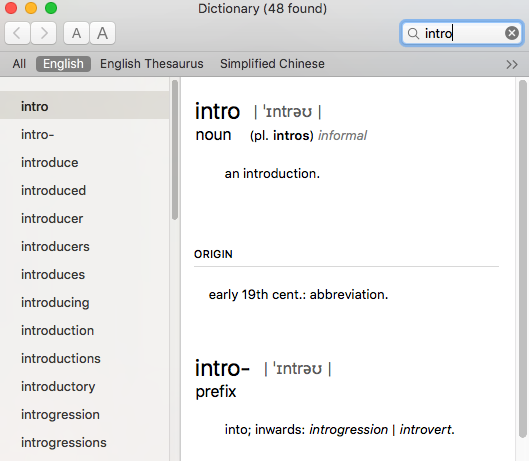
\includegraphics[scale=0.4]{img/edict-en.eps}
  \caption{E-dictionary. All candidates starting with what the user input are listed.}
  \label{fig:e-dict}
\end{figure}

A E-dictionary typically contains hundreds of thousands words. It's very expensive
to perform a complete search. Commercial software adopts complex approaches, including
caching, indexing etc to speed up this process.

Similar with e-dictionary, figure \ref{fig:word-completion} shows a popular
Internet search engine. When user input something, it provides a candidate
lists, with all items starting with what the user has entered\footnote{It's more complex than just matching the prefix. Including the spell checking and auto currection, key words extraction and recommendation etc.}. And these candidates
are shown in the order of popularity. The more people search, the
upper position it is in the list.

\begin{figure}[htbp]
  \centering
  \includegraphics[scale=0.5]{img/adaptive-input.eps}
  \caption{A search engine. All candidates starting with what user input are listed.}
  \label{fig:word-completion}
\end{figure}

In both cases, the software provides a kind of word auto-completion mechanism.
Some editors can also help programmers to auto-complete the code.

Let's see how to implement the e-dictionary with prefix tree.
To simplify the problem, we assume the dictionary only supports English - English
information.

A dictionary stores key-value pairs, the key is English
word or phrase, the value is the meaning described in text.

We can store all the words and their meanings in a trie, but it consumes
too large space especially when there are huge amount of items. We'll use
prefix tree to realize the e-dictionary.

When user wants to look up word 'a', the dictionary does not only
return the meaning of 'a', but also provides a list of
candidates starting with 'a', including 'abandon', 'about',
'accent', 'adam', ... Of course all these words are stored in the prefix tree.

If there are too many candidates, we can limit only displaying the top 10
candidates, and allow the user to browse more.

TODO: Change the order of FP and Imperative

The following algorithm reuses the looking up defined for prefix tree. When
finds a node bound the prefix of what we are looking for,
it expands all its children sub-trees till getting $n$ candidates.

\begin{algorithmic}[1]
\Function{Look-Up}{$T, k, n$}
  \If{$T = $ NIL}
     \State \Return $\phi$
  \EndIf
  \State $prefix \gets$ NIL
  \Repeat
    \State $match \gets$ FALSE
    \For{$\forall (k_i, T_i) \in $ \Call{Children}{$T$}}
      \If{$k$ is prefix of $k_i$}
        \State \Return \Call{Expand}{$T_i, prefix, n$}
      \EndIf
      \If{$k_i$ is prefix of $k$}
        \State $match \gets$ TRUE
        \State $k \gets k - k_i$
        \State $T \gets T_i$
        \State $prefix \gets prefix + k_i$
        \State break
      \EndIf
    \EndFor
  \Until{$\lnot match$}
  \State \Return $\phi$
\EndFunction
\end{algorithmic}

Where function \textproc{Expand}($T, prefix, n$) picks $n$ sub-trees, which
share the same prefix in $T$. It is realized as BFS (Bread-First-Search) traverse. 14.3.1 in the Chapter of search
explains BFS in detail.

\begin{algorithmic}[1]
\Function{Expand}{$T, prefix, n$}
  \State $R \gets \phi$
  \State $Q \gets \{(prefix, T)\}$
  \While{$|R| < n \land |Q| > 0$}
    \State $(k, T) \gets$ \Call{Pop}{$Q$}
    \If{\Call{Data}{$T$} $\neq$ NIL}
      \State $R \gets R \cup \{(k, $ \Call{Data}{$T$} $)\}$
    \EndIf
    \For{$\forall (k_i, T_i) \in$ \Call{Children}{$T$} in sorted order}
      \State \Call{Push}{$Q, (k + k_i, T_i)$}
    \EndFor
  \EndWhile
\EndFunction
\end{algorithmic}

The following example Java program implements the e-dictionary application.

\lstset{language=Java}
\begin{lstlisting}
public <T> List<Map.Entry<String, T>> lookup(PrefixTree.Node<T> t,
                                             String key, int n) {
    if (t == null)
        return Collections.emptyList();
    String prefix = "";
    boolean match;
    do {
        match = false;
        for (Map.Entry<String, PrefixTree.Node<T>> entry : t.subTrees.entrySet()) {
            String k = entry.getKey();
            PrefixTree.Node<T> tr = entry.getValue();
            if (k.startsWith(key)) { // key is prefix of k
                return expand(prefix + k, tr, n);
            }
            if (key.startsWith(k)) {
                match = true;
                key = key.substring(k.length());
                t = tr;
                prefix = prefix + k;
                break;
            }
        }
    } while (match);
    return Collections.emptyList();
}

<T> List<Map.Entry<String, T>> expand(String prefix, PrefixTree.Node<T> t, int n) {
    List<Map.Entry<String, T>> res = new ArrayList<>();
    Queue<Map.Entry<String, PrefixTree.Node<T> >> q = new LinkedList<>();
    q.offer(entryOf(prefix, t));
    while(res.size() < n && !q.isEmpty()) {
        Map.Entry<String, PrefixTree.Node<T>> entry = q.poll();
        String s = entry.getKey();
        PrefixTree.Node<T> tr = entry.getValue();
        if (tr.value.isPresent()) {
            res.add(entryOf(s, tr.value.get()));
        }
        for (Map.Entry<String, PrefixTree.Node<T>> e :
                 new TreeMap<>(tr.subTrees).entrySet()) {
            q.offer(entryOf(s + e.getKey(), e.getValue()));
        }
    }
    return res;
}

<K, V> Map.Entry<K, V> entryOf(K key, V val) {
    return new AbstractMap.SimpleImmutableEntry<K, V>(key, val);
}
\end{lstlisting}

This algorithm can also be implemented recursively, if the string we
are looking for is empty, we expand all children until getting $n$
candidates. Otherwise we recursively examine the children to
find one which has prefix equal to this string.

In programming environments supporting lazy evaluation. An intuitive
solution is to expand all candidates, and take the first $n$ on
demand. Denote the prefix tree in form $T = (v, C)$,
below function enumerates all items starts with key $k$.

\be
findAll(T, k) = \left \{
  \begin{array}
  {r@{\quad:\quad}l}
  enum(C) & k = \phi, v = \phi \\
  \{(\phi, v)\} \cup enum(C) & k = \phi, v \neq \phi \\
  find(C, k) & k \neq \phi
  \end{array}
\right.
\ee

The first two clauses deal with the edge cases the the key is empty.
All the children are enumerated except for those with empty values.
The last clause finds child matches $k$.

For non-empty children, $C = \{(k_1, T_1), (k_2, T_2), ..., (k_m, T_m)\}$,
denote the rest pairs except for the first one as $C'$.
The enumeration algorithm can be defined as below.

\be
enum(C) = \left \{
  \begin{array}
  {r@{\quad:\quad}l}
  \phi & C = \phi \\
  mapAppend(k_1, findAll(T_1, \phi)) \cup enum(C')
  \end{array}
\right.
\ee

Where $mapAppend(k, L) = \{(k + k_i, v_i)| (k_i, v_i) \in L\}$. It concatenate
the prefix $k$ in front of every key-value pair in list $L$.

Function $find(C, k)$ is defined as the following. For empty children, the
result is empty as well; Otherwise, it examines the first child $T_1$ which
is bound to string $k_1$. If $k_1$ is equal to $k$, it calls $mapAppend$ to
add prefix to the keys of all the children under $T_1$; If $k_1$ is prefix
of $k$, the algorithm recursively find all children start with $k - k_1$;
On the other hand, if $k$ is prefix of $k_1$, all children under $T_1$
are valid result. Otherwise, the algorithm by-pass the first child
and goes on find the rest children.

\be
find(C, k) = \left \{
  \begin{array}
  {r@{\quad:\quad}l}
  \phi & C = \phi \\
  mapAppend(k, findAll(T_1, \phi)) & k_1 = k \\
  mapAppend(k_1, findAll(T_1, k - k_1)) & k_1 \sqsubset k \\
  findAll(T_1, \phi) & k \sqsubset k_1 \\
  find(C', k) & otherwise
  \end{array}
\right.
\ee

Below example Haskell program implements the e-dictionary application
according to the above equations.

\lstset{language=Haskell}
\begin{lstlisting}
findAll :: Patricia a -> Key -> [(Key, a)]
findAll t [] =
    case value t of
      Nothing -> enum $ children t
      Just x  -> ("", x):(enum $ children t)
    where
      enum [] = []
      enum (p:ps) = (mapAppend (fst p) (findAll (snd p) [])) ++ (enum ps)
findAll t k = find' (children t) k where
    find' [] _ = []
    find' (p:ps) k
          | (fst p) == k
              = mapAppend k (findAll (snd p) [])
          | (fst p) `Data.List.isPrefixOf` k
              = mapAppend (fst p) (findAll (snd p) (k `diff` (fst p)))
          | k `Data.List.isPrefixOf` (fst p)
              = findAll (snd p) []
          | otherwise = find' ps k
    diff x y = drop (length y) x

mapAppend s lst = map (\p->(s++(fst p), snd p)) lst
\end{lstlisting}

In the lazy evaluation environment, the top $n$ candidates can be
gotten like $take(n, findAll(T, k))$. Appendix A has detailed definition
of $take$ function.

%=====================================
% T9
%=====================================

\subsection{T9 input method}
\index{T9}
\index{Textonym input method}

Most mobile phones around year 2000 are equipped with a key pad.
Users have quite different experience from PC when editing a short message
or email.
This is because the mobile-phone key pad, or so called ITU-T key pad has much fewer
keys than PC. Figure \ref{fig:itut-keypad} shows one example.

\begin{figure}[htbp]
  \centering
  \includegraphics[scale=0.4]{img/itu-t.eps}
  \caption{an ITU-T keypad for mobile phone.}
  \label{fig:itut-keypad}
\end{figure}

There are typical two methods to input English word or phrases with ITU-T key pad.
For instance, if user wants to enter a word `home', He can press the key
in below sequence.

\begin{itemize}
\item Press key '4' twice to enter the letter 'h';
\item Press key '6' three times to enter the letter 'o';
\item Press key '6' to enter the letter 'm';
\item Press key '3' twice to enter the letter 'e';
\end{itemize}

Another much quicker way is to just press the following keys.

\begin{itemize}
\item Press key '4', '6', '6', '3', word `home' appears on top of the candidate list;
\item Press key '*' to change a candidate word, so word `good' appears;
\item Press key '*' again to change another candidate word, next word `gone' appears;
\item ...
\end{itemize}

Compare these two methods, we can see the second one is much easier for the end user.
The only overhead is to store a dictionary of candidate words.

Method 2 is called as `T9' input method, or predictive input method
\cite{wiki-t9}, \cite {wiki-predictive-text}. The abbreviation 'T9' stands
for 'textonym'. It start with 'T' with 9 characters. T9 input can also be
realized with trie or prefix tree.

In order to provide candidate words to user, a dictionary must be prepared
in advance. Trie or prefix tree can be used to store the dictionary. The
commercial T9 implementations typically use complex indexing dictionary in
both file system and cache. The realization shown here is for illustration
purpose only.

Firstly, we need define the T9 mapping, which maps from digit to candidate
characters.

\be
\begin{array}{ll}
M_{T9} = \{ & 2 \rightarrow abc, 3 \rightarrow def, 4 \rightarrow ghi, \\
           & 5 \rightarrow jkl, 6 \rightarrow mno, 7 \rightarrow pqrs, \\
           & 8 \rightarrow tuv, 9 \rightarrow wxyz \}
\end{array}
\ee

With this mapping, $M_{T9}[i]$ returns the corresponding characters for digit $i$.

Suppose user input digits $D = d_1d_2...d_n$, If $D$ isn't empty, denote the
rest digits except for $d_1$ as $D'$,
below pseudo code shows how to realize T9 with trie.

\begin{algorithmic}[1]
\Function{Look-Up-T9}{$T, D$}
  \State $Q \gets \{(\phi, D, T)\}$
  \State $R \gets \phi$
  \While{$Q \neq \phi$}
    \State $(prefix, D, T) \gets$ \Call{Pop}{$Q$}
    \For{each $c$ in $M_{T9}[d_1]$}
      \If{$c \in $ \Call{Children}{$T$}}
        \If{$D' = \phi$}
          \State $R \gets R \cup \{prefix + c\}$
        \Else
          \State \textproc{Push}($Q, (prefix + c, D', $ \Call{Children}{$t$}$[c])$)
        \EndIf
      \EndIf
    \EndFor
  \EndWhile
  \State \Return $R$
\EndFunction
\end{algorithmic}

Where $prefix + c$ means appending character $c$ to the end of string $prefix$.
Again, this algorithm performs BFS search with a queue $Q$. The queue is
initialized with a tuple $(prefix, D, T)$, containing empty prefix, the digit sequence to be
searched, and the trie. It keeps picking the tuple from the queue as far as
it isn't empty. Then get the candidate characters from the first digit to
be processed via the T9 map. For each character $c$, if there is a sub-tree
bound to it, we created a new tuple, update the prefix by appending $c$,
using the rest of digits to update $D$, and use that sub-tree. This new tuple
is pushed back to the queue for further searching. If all the digits are
processed, it means a candidate word is found. We put this word to the
result list $R$.

The following example program in Python implements this T9 search with trie.

\lstset{language=Python}
\begin{lstlisting}
T9MAP={'2':"abc", '3':"def", '4':"ghi", '5':"jkl", \
       '6':"mno", '7':"pqrs", '8':"tuv", '9':"wxyz"}

def trie_lookup_t9(t, key):
    if t is None or key == "":
        return None
    q = [("", key, t)]
    res = []
    while len(q)>0:
        (prefix, k, t) = q.pop(0)
        i=k[0]
        if not i in T9MAP:
            return None #invalid input
        for c in T9MAP[i]:
            if c in t.children:
                if k[1:]=="":
                    res.append((prefix+c, t.children[c].value))
                else:
                    q.append((prefix+c, k[1:], t.children[c]))
    return res
\end{lstlisting}

Because trie is not space effective, we can modify the above algorithm with
prefix tree solution. As far as the queue isn't empty, the algorithm pops the
tuple. This time, we examine all the (prefix, sub-tree) pairs. For every pair
$(k_i, T_i)$, we convert the alphabetic prefix $k_i$ back to digits sequence $D'$
by looking up the T9 map. If $D'$ exactly matches the digits of what user input,
we find a candidate word; otherwise if the digit sequence is prefix of what user inputs,
the program creates a new tuple, updates the prefix, the digits to be processed,
and the sub-tree. Then put the tuple back to the queue for further search.

\begin{algorithmic}[1]
\Function{Look-Up-T9}{$T, D$}
  \State $Q \gets \{(\phi, D, T)\}$
  \State $R \gets \phi$
  \While{$Q \neq \phi$}
    \State $(prefix, D, T) \gets$ \Call{Pop}{$Q$}
    \For{each $(k_i, T_i) \in $ \Call{Children}{$T$}}
      \State $D' \gets$ \Call{Convert-T9}{$k_i$}
      \If{$D' \sqsubset D$} \Comment{$D'$ is prefix of $D$}
        \If{$D' = D$}
          \State $R \gets R \cup \{prefix + k_i\}$
        \Else
          \State \textproc{Push}($Q, (prefix + k_i, D - D', T_i)$)
        \EndIf
      \EndIf
    \EndFor
  \EndWhile
  \State \Return $R$
\EndFunction
\end{algorithmic}

Function \textproc{Convert-T9}($K$) converts each character in $K$ back to digit.

\begin{algorithmic}[1]
\Function{Convert-T9}{$K$}
  \State $D \gets \phi$
  \For{each $c \in K$}
     \For{each $(d \rightarrow S) \in M_{T9}$}
       \If{$c \in S$}
         \State $D \gets D \cup \{d\}$
         \State break
       \EndIf
     \EndFor
  \EndFor
  \State \Return $D$
\EndFunction
\end{algorithmic}

The following example Python program implements the T9 input method with prefix tree.

\lstset{language=Python}
\begin{lstlisting}
def patricia_lookup_t9(t, key):
    if t is None or key == "":
        return None
    q = [("", key, t)]
    res = []
    while len(q)>0:
        (prefix, key, t) = q.pop(0)
        for k, tr in t.children.items():
            digits = toT9(k)
            if string.find(key, digits)==0: #is prefix of
                if key == digits:
                    res.append((prefix+k, tr.value))
                else:
                    q.append((prefix+k, key[len(k):], tr))
    return res
\end{lstlisting}

T9 input method can also be realized recursively. Let's first define
the trie solution. The algorithm takes two arguments, a trie storing
all the candidate words, and a sequence of digits that is input by
the user. If the sequence is empty, the result is empty as well;
Otherwise, it looks up $C$ to find those children which are bound
to the first digit $d_1$ according to T9 map.

\be
findT9(T, D) = \left \{
  \begin{array}
  {r@{\quad:\quad}l}
  \{ \phi \} & D = \phi \\
  fold(f, \phi, lookupT9(d_1, C)) & otherwise
  \end{array}
\right.
\ee

Where folding is defined in Appendix A. Function $f$ takes two arguments,
an intermediate list of candidates which is initialized empty, and
a pair $(c, T')$, where $c$ is candidate character, to which sub-tree $T'$
is bound. It append character $c$ to all the candidate words, and concatenate
this to the result list.

\be
f(L, (c, T')) = mapAppend(c, findT9(T', D')) \cup L
\ee

Note this $mapAppend$ function is a bit different from the previous one defined
in e-dictionary application. The first argument is a character, but not a string.

Function $lookupT9(k, C)$ checks all the possible characters mapped to digit $k$.
If the character is bound to some child in $C$, it is record as one candidate.

\be
lookupT9(k, C) =  fold(g, \phi, M_{T9}[k])
\ee

Where

\be
g(L, k) = \left \{
  \begin{array}
  {r@{\quad:\quad}l}
  L & find(C, k) = \phi \\
  \{(k, T')\} \cup L & find(C, k) = T'
  \end{array}
\right.
\ee

Below Haskell example program implements the T9 look up algorithm with trie.

\lstset{language=Haskell}
\begin{lstlisting}
mapT9 = [('2', "abc"), ('3', "def"), ('4', "ghi"), ('5', "jkl"),
         ('6', "mno"), ('7', "pqrs"), ('8', "tuv"), ('9', "wxyz")]

findT9 t [] = [("", value t)]
findT9 t (k:ks) = foldl f [] (lookupT9 k (children t))
    where
      f lst (c, tr) = (mapAppend' c (findT9 tr ks)) ++ lst

lookupT9 c children = case lookup c mapT9 of
        Nothing -> []
        Just s  -> foldl f [] s where
             f lst x = case lookup x children of
                 Nothing -> lst
                 Just t  -> (x, t):lst

mapAppend' x lst = map (\p->(x:(fst p), snd p)) lst
\end{lstlisting}

There are few modifications when change the realization from trie to prefix tree.
Firstly, the sub-tree is bound to prefix string, but not a single character.

\be
findT9(T, D) = \left \{
  \begin{array}
  {r@{\quad:\quad}l}
  \{ \phi \} & D = \phi \\
  fold(f, \phi, findPrefixT9(D, C)) & otherwise
  \end{array}
\right.
\ee

The list for folding is given by calling function $findPrefixT9(D, C)$.
And $f$ is also modified to reflect this change. It appends the
candidate prefix $D'$ in front of every result output by the
recursive search, and then accumulates the words.

\be
f(L, (D', T')) = mapAppend(D', findT9(T', D - D')) \cup L
\ee

Function $findPrefixT9(D, C)$ examines all the children. For
every pair $(k_i, T_i)$, if converting $k_i$ back to digits
yields a prefix of $D$, then this pair is selected as a
candidate.

\be
findPrefixT9(D, C) = \{ (k_i, T_i) |(k_i, T_i) \in C, convertT9(k_i) \sqsubset D\}
\ee

Function $convertT9(k)$ converts every alphabetic character in $k$ back
to digits according to T9 map.

\be
convertT9(K) = \{ d | \forall c \in k, \exists (d \rightarrow S) \in M_{T9} \Rightarrow c \in S\}
\ee

The following example Haskell program implements the T9 input algorithm
with prefix tree.

\begin{lstlisting}
findT9 t [] = [("", value t)]
findT9 t k = foldl f [] (findPrefixT9 k (children t))
    where
      f lst (s, tr) = (mapAppend s (findT9 tr (k `diff` s))) ++ lst
      diff x y = drop (length y) x

findPrefixT9 s lst = filter f lst where
    f (k, _) = (toT9 k) `Data.List.isPrefixOf` s

toT9 = map (\c -> head $ [ d |(d, s) <- mapT9, c `elem` s])
\end{lstlisting}

\begin{Exercise}
\begin{itemize}
\item For the T9 input, compare the results of the algorithms realized with trie and prefix tree,
the sequences are different. Why does this happen? How to modify the algorithm so that they
output the candidates with the same sequence?
\end{itemize}
\end{Exercise}

% ================================================================
%                 Short summary
% ================================================================
\section{Summary}

In this chapter, we start from the integer base trie and prefix tree. The
map data structure based on integer tree plays an important role
in Compiler implementation. Alphabetic trie and prefix tree are
natural extensions. They can be used to manipulate text information.
As examples, predictive e-dictionary and T9 input method are
realized with trie or prefix tree. Although these examples
are different from the real implementation in commercial software.
They show simple approaches to solve some problems.
Other important data structure, such as suffix tree, has close
relationship with them. Suffix tree is introduced in the next chapter.

\begin{thebibliography}{99}

\bibitem{CLRS}
Thomas H. Cormen, Charles E. Leiserson, Ronald L. Rivest and Clifford Stein.
``Introduction to Algorithms, Second Edition''. Problem 12-1. ISBN:0262032937. The MIT Press. 2001

\bibitem{okasaki-int-map}
Chris Okasaki and Andrew Gill. ``Fast Mergeable Integer
Maps''. Workshop on ML, September 1998, pages 77-86, \url{http://www.cse.ogi.edu/~andy/pub/finite.htm}

\bibitem{patricia-morrison}
D.R. Morrison, ``PATRICIA -- Practical Algorithm To Retrieve  Information Coded In Alphanumeric", Journal of the ACM, 15(4), October 1968, pages 514-534.

\bibitem{wiki-suffix-tree}
Suffix Tree, Wikipedia. \url{http://en.wikipedia.org/wiki/Suffix_tree}

\bibitem{wiki-trie}
Trie, Wikipedia. \url{http://en.wikipedia.org/wiki/Trie}

\bibitem{wiki-t9}
T9 (predictive text), Wikipedia. \url{http://en.wikipedia.org/wiki/T9_(predictive_text)}

\bibitem{wiki-predictive-text}
Predictive text,
Wikipedia. \url{http://en.wikipedia.org/wiki/Predictive_text}

\end{thebibliography}

\ifx\wholebook\relax\else
\end{document}
\fi
